\documentclass[twocolumn,amsmath,amssymb,floatfix]{revtex4}

\usepackage{graphicx}% Include figure files
\usepackage{dcolumn}% Align table columns on decimal point
\usepackage{bm}% bold math
\usepackage{amssymb}
\usepackage{amsmath}
\usepackage{amsfonts}
\usepackage{epsf}
\usepackage{color} % allows color in fonts
\usepackage{verbatim}
\usepackage{listings}
\usepackage{xcolor}
\usepackage{titlesec}
\usepackage{float}

\usepackage[brazilian]{babel}
\usepackage[utf8]{inputenc}
\usepackage[T1]{fontenc}

\newcommand{\PAR}[1]{\left({[#1]}\right)}


\lstdefinestyle{customc}{
  belowcaptionskip=1\baselineskip,
  breaklines=true,
  frame=none,
  xleftmargin=\parindent,
  language=C,
  showstringspaces=false,
  basicstyle=\footnotesize\ttfamily,
  keywordstyle=\bfseries\color{green!40!black},
  commentstyle=\itshape\color{purple!40!black},
  identifierstyle=\color{blue},
  stringstyle=\color{orange},
}

\lstdefinestyle{customasm}{
  belowcaptionskip=1\baselineskip,
  frame=trBL,
  xleftmargin=\parindent,
  language=[x86masm]Assembler,
  basicstyle=\footnotesize\ttfamily,
  commentstyle=\itshape\color{purple!40!black},
}

\lstset{escapechar=@,style=customc}

\titlespacing\section{0pt}{12pt plus 4pt minus 2pt}{8pt plus 2pt minus 2pt}
\titlespacing\subsection{0pt}{12pt plus 4pt minus 2pt}{8pt plus 2pt minus 2pt}
\titlespacing\subsubsection{0pt}{12pt plus 4pt minus 2pt}{0pt plus 2pt minus 2pt}

\begin{document}

%%%%%%%%%%%%%%%%%%%%%%
%%%%%%%%%%%%%%%%%%%%%%
% T I T U L O
%%%%%%%%%%%%%%%%%%%%%%
%%%%%%%%%%%%%%%%%%%%%%

\title{Relatorio Exercicio Computacional 3}

\author{Leonardo Heidi Almeida Murakami - NUSP: 11260186 \\\small leonardo.murakami@usp.br} 
\affiliation{
Instituto de Matemática e Estatística - Universidade de São Paulo\\
}

\begin{abstract}
\baselineskip 11pt
Neste trabalho estudaremos a diferença de eficiencia na utilização de numeros quasi-aleatórios quando comparados com número verdadeiramente aleatórios na convergência de métodos Monte Carlo. Para isso utilizaremos os métodos introduzidos no EP2 e compararemos os seus resultados.
\end{abstract}

\maketitle
%%%%%%%%%%%%%%%%%%%%%%
%%%%%%%%%%%%%%%%%%%%%%
\section{Introdução e Conceitos}
%%%%%%%%%%%%%%%%%%%%%%
%%%%%%%%%%%%%%%%%%%%%%

\indent Os métodos de Monte Carlo são uma classe ampla de algoritmos computacionais que dependem de uma amostragem aleatória para obter resultados numéricos. 
\\\indent A ideia para obtermos o valor de 
\begin{eqnarray}
  \int^1_0 exp(0.394353985x)*cos(0.50451412877x)
\end{eqnarray}
sera nos utilizarmos de 4 métodos diferentes de Monte Carlo. \\
\indent O conceito de Monte Carlo continua igual ao introduzido anteriormente, desta vez, porém, utilizaremos um método diferente para gerarmos os números aleatórios, utilizaremos uma sequencia de Halton para gerarmos pontos em nosso espaço.
\subsection{Sequencia de Halton}
\indent Apesar de ser uma sequência determinística, as sequencias de Halton apresentam baixa discrepância, ou seja, aparentam ser aleatórias. No nosso caso elas apresentam a vantagem de serem mais uniformemente distribuídas no espaço, causando uma convergência mais rápida dos métodos MC
\subsection{Hit or Miss Monte Carlo}
\indent O Método Hit or Miss sofre poucas mudanças em sua implementação com o gerador de número quasi-aleatórios. Como estamos gerando números com o parametro de dimensão em 2 obtemos as coordenadas x e y imediatamente.
\subsection{Crude Monte Carlo}
\indent O Método Crude também sofre poucas mudanças. Em geral a única mudança que acontece no algoritmo é a geração da sequencia de Halton no começo da implementação e ignorarmos a segunda dimensão gerada, pegamos então o número dado pela sequência e rodamos o algoritmo normalmente.
\subsection{Importance Sampling}
\indent O Importance Sampling foi alterado de modo a pegar o valor gerado pela sequência (de 0 a 1) e gerar a sua probabilidade de X para cada distribuição passada ao algoritmo. Pegamos então essa probabilidade de X como o valor aleátório gerado pela distribuição e rodamos o resto do algoritmo normalmente.
\subsection{Control Variates}
\indent O método de redução de variância foi trocado apenas o gerador aleatório, a função usada para aproximar a integral foi a mesma. \\
\indent Onde, neste caso, a função usada para reduzir o erro da nossa integral foi
\begin{eqnarray}
  g(x) = -0.4x + 1
\end{eqnarray}
%%%%%%%%%%%%%%%%%%%%%%
%%%%%%%%%%%%%%%%%%%%%%
\section{Implementação e testes}
%%%%%%%%%%%%%%%%%%%%%%
%%%%%%%%%%%%%%%%%%%%%%

\indent Os algoritmos foram implementados na linguagem Python 3.8, organizado em 3 arquivo: \textit{monte\_carlo\_methods.py}, \textit{qng\_monte\_carlo\_methods.py} e \text{compare\_methods.py}. \\
\indent Os gráficos foram gerados usando a biblioteca \textit{matplotlib} do Python e utilizando a interface web do \textit{Wolfram|Alpha}, as distribuções foram geradas utilizando a biblioteca \textit{SciPy}, a algebra com vetores foi otimizada utilizando-se da biblioteca \textit{NumPy} e para gerar a sequencia de números quasi-aleatórios (sequencia de Halton) utilizei a biblioteca \textit{Ghalton}, todas elas estão disponiveis no package manager comum do python (PyPI). As partes relevantes dos códigos podem ser conferidos no próprio arquivo enviado junto com este PDF/Tex.

%%%%%%%%%%%%%%%%%%%%%%
\subsection{Arquivos do projeto}
%%%%%%%%%%%%%%%%%%%%%%
Abaixo segue um breve resumo do conteúdo dos códigos fonte e interfaces.
\\\indent \textbf{monte\_carlo\_methods.py:} Implementa o algoritmo visto no EP2. Um pedaço de sua interface é apresentado a seguir:
\begin{lstlisting}
def generate_point() -> Tuple(float, float):

def generate_values(dist: Scipy.distribution, size: int=30000) -> List(float):

def crude_monte_carlo(f_x: Function, n_samples: int) -> float:

def hit_or_miss_monte_carlo(f_x: Function, n_samples: int) -> float:

def importance_sampling_monte_carlo(distribution: Scipy.distribution, f_x: Function, n_samples: int) -> float:

def control_variates_monte_carlo(control_variate: Function, gamma_integrated_control_variate: float, f_x: Function, n_samples: int) -> float:

def estimate_error(monte_carlo_algorithm: function, f_x: function, n_batches: int, distribution: Scipy.distribution, control_variate: function, gamma_integrated_control_variate: float) -> List(float), float:

def main() -> None
\end{lstlisting}
\\\indent \textbf{qng\_monte\_carlo\_methods.py:} Implementa o algoritmo visto no EP2 com números quasi-aleatórios. Um pedaço de sua interface é apresentado a seguir:
\begin{lstlisting}
def generate_points(n_points) -> List[Tuple(float, float)]:

def generate_quasi_random_point(): -> float

def generate_values(dist: Scipy.distribution, size: int=30000) -> List(float):

def crude_monte_carlo(f_x: Function, n_samples: int) -> float:

def hit_or_miss_monte_carlo(f_x: Function, n_samples: int) -> float:

def importance_sampling_monte_carlo(distribution: Scipy.distribution, f_x: Function, n_samples: int) -> float:

def control_variates_monte_carlo(control_variate: Function, gamma_integrated_control_variate: float, f_x: Function, n_samples: int) -> float:

def estimate_error(monte_carlo_algorithm: function, f_x: function, n_batches: int, distribution: Scipy.distribution, control_variate: function, gamma_integrated_control_variate: float) -> List(float), float:

def main() -> None
\end{lstlisting}
\\\indent \textbf{compare\_methods.py:} Compara os metodos de Monte Carlo implementados em cada arquivo e ao rodar a main, salva os graficos comparando os algoritmos:
\begin{lstlisting}
def estimate_error(monte_carlo_algorithm: function, f_x: function, n_batches: int, distribution: Scipy.distribution, control_variate: function, gamma_integrated_control_variate: float) -> List(float), float:

def compare_methods(method_1: function, method_2: function, estimate_error_args: dict, figname: str) -> None

def main() -> None
\end{lstlisting}
%%%%%%%%%%%%%%%%%%%%%%
\subsection{Algoritmo}
%%%%%%%%%%%%%%%%%%%%%%
\indent A implementação do algoritmo em questão é apresentado abaixo. As funções com o nome de monte\_carlo são passadas como argumento para a função estimate\_error que recebe como argumento os argumentos necessarios para que todos os metodos de Monte Carlo rodem com sucesso, os $N$ foram definidos como constantes no começo do código assim como o valor $M$, que é o numero de vezes que cada algoritmo de Monte Carlo ira rodar para podermos calcular um erro
\begin{lstlisting}
def main():
  errors_crude, estimated_value_crude = estimate_error(crude_monte_carlo, f_x)
  print("-"*4 + "CRUDE MONTE CARLO" + "-"*4)
  print(f"Mean Error: \t {np.mean(errors_crude)}")
  print(f"Estimated Value: \t {estimated_value_crude}")

  errors_hom, estimated_value_hom = estimate_error(hit_or_miss_monte_carlo, f_x)
  print("-"*4 + "HIT OR MISS MONTE CARLO" + "-"*4)
  print(f"Mean Error: \t {np.mean(errors_hom)}")
  print(f"Estimated Value: \t {estimated_value_hom}")

  isc_errors, isc_estimated_value = estimate_error(importance_sampling_monte_carlo, f_x, distribution=stats.beta(a=1, b=1.2))
  print("-"*4 + "BETA DISTRIBUTION IMPORTANCE SAMPLING MONTE CARLO" + "-"*4)
  print(f"Mean Error: \t {np.mean(isc_errors)}")
  print(f"Estimated Value: \t {isc_estimated_value}")

  isc_errors, isc_estimated_value = estimate_error(importance_sampling_monte_carlo, f_x, distribution=stats.gamma(a=1, scale=1.4))
  print("-"*4 + "GAMMA DISTRIBUTION IMPORTANCE SAMPLING MONTE CARLO" + "-"*4)
  print(f"Mean Error: \t {np.mean(isc_errors)}")
  print(f"Estimated Value: \t {isc_estimated_value}")

  isc_errors, isc_estimated_value = estimate_error(importance_sampling_monte_carlo, f_x, distribution=stats.weibull_min(c=1, scale=1.1))
  print("-"*4 + "WEIBULL DISTRIBUTION IMPORTANCE SAMPLING MONTE CARLO" + "-"*4)
  print(f"Mean Error: \t {np.mean(isc_errors)}")
  print(f"Estimated Value: \t {isc_estimated_value}")
  
  control_variate = lambda x: -0.4*x + 1
  gamma_integrated_control_variate = 0.8
  control_variate_errors, control_variate_estimated_value = estimate_error(
      control_variates_monte_carlo, f_x, 
      control_variate = control_variate,
      gamma_integrated_control_variate = gamma_integrated_control_variate
      )
  print("-"*4 + "CONTROL VARIATES MONTE CARLO" + "-"*4)
  print(f"Mean Error: \t {np.mean(control_variate_errors)}")
  print(f"Estimated Value: \t {control_variate_estimated_value}")
\end{lstlisting}
\indent A função main em cada arquivo é utilizada para rodarmos todos os algoritmos dentro da função estimate error para gerarmos os valores estimados e erros, todos os atributos de distribuições, assim como a função do método Control Variates estão definidos dentro da main e podem ser alterados sem muita dificuldade \\
\indent A maior parte do algoritmo de comparação esta encapsulado dentro da função compare\_methods que salva os gráficos que serão apresentados a baixo, ela calcula o valor médio estimado até aquele passo do programa e depois monta um gráfico com esses valores para ver a convergência ao longo do tempo.
\begin{lstlisting}
def compare_methods(method_1, method_2, estimate_error_args={}, figname=None):
    def rolling_average(list):
        average_till_point = []
        for i in range(1, len(list)):
            average_till_point.append(np.mean(list[:i]))
        return average_till_point

    qng_errors_crude, qng_values_crude = estimate_error(method_1, f_x, **estimate_error_args)
    mcm_errors_crude, mcm_values_crude = estimate_error(method_2, f_x, **estimate_error_args)

    qng_plot_list = rolling_average(qng_values_crude)
    mcm_plot_list = rolling_average(mcm_values_crude)
    fig = plt.figure()
    plt.plot(qng_plot_list, label='Quasi-random Number Generator MCM')
    plt.plot(mcm_plot_list, c='red', label='Random MCM')
    fig.savefig(figname)
\end{lstlisting}
%%%%%%%%%%%%%%%%%%%%%%
\subsection{Conclusão}
%%%%%%%%%%%%%%%%%%%%%%
\indent No geral, todos os algoritmos funcionam melhor quando funcionando sobre números quasi-aleatórios, eles funcionam extremamente mais rápidos, com métodos (tipo o de control variates) convergindo em pouquíssimos batches.\\
\indent Com os gráficos gerados pelo programa, conseguimos entender um pouco melhor a melhora de eficiência para cada algoritmo (MCM = Monte Carlo Method).\\
\subsubsection{Crude Monte Carlo}
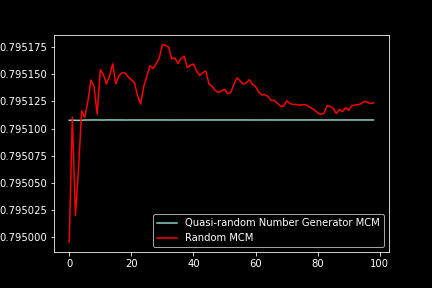
\includegraphics[scale=0.55]{CrudeComparison.png}
\indent Podemos observar facilmente que, embora os valores sejam muito próximos (apresentado pelo eixo Y) os valores estimados pelos valores quasi-aleatórios convergem muito mais rapidamente (indicado pela linha praticamente reta)
\subsubsection{Hit or Miss Monte Carlo}
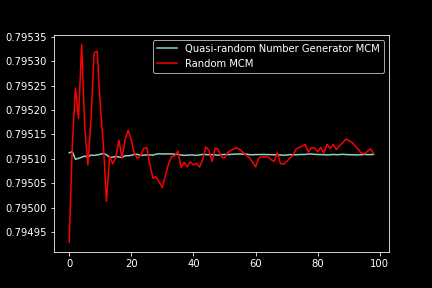
\includegraphics[scale=0.55]{HitOrMissComparison.png}
\indent O comportamento se repete na maioria dos casos, onde a convergência é atingida rapidamente pelo gerador quasi-aleatório, isso pode ser dado principalmente pelo comportamento mais uniforme entre os pontos.
\vfill\null
\columnbreak
\subsubsection{Importance Sampling}
\indent Podemos observar abaixo o mesmo comportamento em todos os gráficos, podemos sempre concluir que a convergência e atingida mais rápido pelo método Quasi-random por apresentar pouca mudança uma vez que atinge um certo valor, onde o pseudo-aleatório fica alternando entre valores próximos
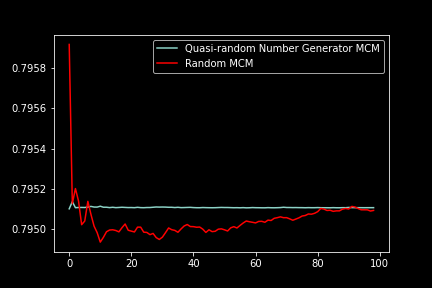
\includegraphics[scale=0.55]{BetaImportanceSamplingComparison.png}
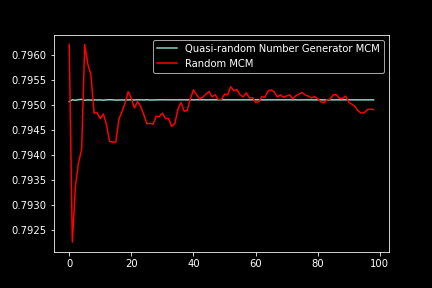
\includegraphics[scale=0.55]{GammaImportanceSamplingComparison.png}
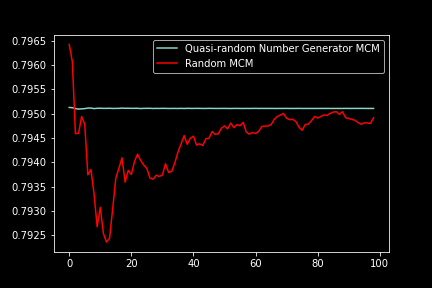
\includegraphics[scale=0.55]{WeibullImportanceSamplingComparison.png}
\subsubsection{Control Variates}
\indent Como esse método recebia números menores para o método pseudo-aleatório, e possível ver a pequena convergência do método quasi-aleatório.
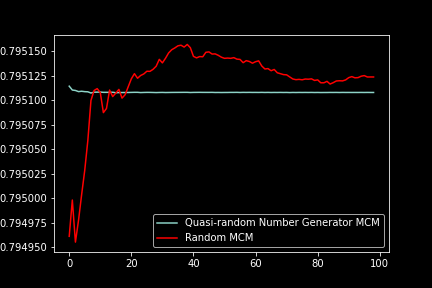
\includegraphics[scale=0.55]{ControlVariatesComparison.png}
\subsubsection{Comparação Geral}
\indent Aqui compararei os valores necessários de $N$ e $M$ para atingirmos o erro desejado no ultimo exercício computacional (de 0.0005). A tabela embaixo mostra o quão mais eficiente são os métodos de Monte Carlo quando pareados a um gerador de numero quasi-aleatórios, isso é dado no geral pela melhor "ocupação" do espaço pelos números quasi-aleatórios
\begin{center}
 \begin{tabular}{||c c c c||} 
 \hline
 Algoritmo pseudo-randômico & N & M & N Total \\ [0.5ex] 
 \hline\hline
 Crude & 300000 & 100 & 30000000 \\ 
 \hline
 Hit or Miss & 400000 & 100 & 40000000 \\
 \hline
 Importance Sampling & 25000 & 100 & 2500000 \\
 \hline
 Control Variates & 1000 & 100 & 100000 \\
 \hline
\end{tabular}
\end{center}
\begin{center}
 \begin{tabular}{||c c c c||} 
 \hline
 Algoritmo quasi-randômico & N & M & N Total \\ [0.5ex] 
 \hline\hline
 Crude & 3000 & 100 & 300000 \\ 
 \hline
 Hit or Miss & 4000 & 100 & 400000 \\
 \hline
 Importance Sampling & 2500 & 100 & 250000 \\
 \hline
 Control Variates & 10 & 100 & 1000 \\
 \hline
\end{tabular}
\end{center}
\end{document}